\section{Experiments}
\label{sec:experiments}
\begin{figure}
    \centering
    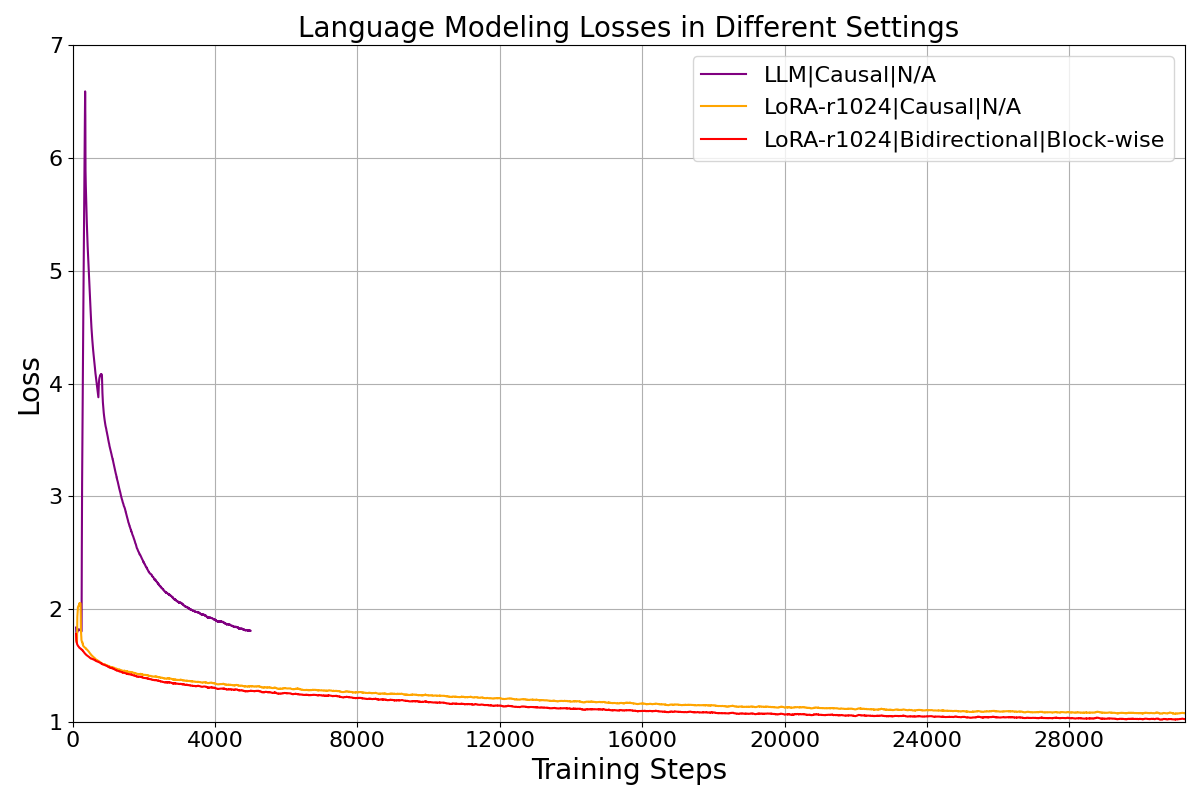
\includegraphics[width=\linewidth]{images/loss_curves_full_llm.png}
    \caption{Language modeling losses in different settings. Training the full LLM with a new modality of data can lead to unrecoverable spike in loss curve, i.e., loss collapse.}
    \label{fig:full_llm}
\end{figure}
\subsection{Implementation details}
\textbf{Training setup.}
Unless otherwise specified, we employed AIMv2-Huge-448p \cite{aimv2} as the default vision encoder and Qwen2.5-7B-Instruct \cite{qwen2.5} as the LLM across all experiments. The pre-training learning rate was fixed at 0.0002 (held constant unless explicitly varied), with 100 warm-up steps and a global batch size maintained at 256. All other hyperparameters and optimizer configurations followed the defaults in \cite{llava1_5}. 

For fine-tuning, all LoRA layers were merged into the LLM, while other components (e.g., distillation modules) were eliminated. The full LLM and 6M-parameter visual embedding layer were trainable. For native-resolution variants (\model{}-AnyRes in Table \ref{tab:ablation}), we retained the pre-trained weights of the fixed-resolution version and adopted native-resolution strategy only during fine-tuning.
\\
\textbf{Benchmarks.} As shown in Table \ref{tab:ablation} and Table \ref{tab:mlm_comparison}, we evaluated the model on several benchmarks: VQAv2: VQAv2 \cite{vqav2}; SQA-I: ScienceQA-Image \cite{scienceqa}; TQA: TextVQA \cite{textvqa}; POPE: POPE \cite{pope}; $\mathrm{MMP_p}$: MME Perception \cite{mme}; $\mathrm{MME_c}$: MME Cognition \cite{mme}; MMB: MMBench \cite{mmbench}; SEED-I: SEED-Image \cite{seed}; MMVet: MMVet \cite{mmvet}; AI2D: AI2D \cite{ai2d}; RQA: Realworld-QA \cite{grok1.5v}; MMMU: MMMU \cite{mmmu}.
% \textbf{Pre-training configurations.} 
% Unless otherwise specified, we employed AIMv2-Huge-448p as our default ViT and Qwen2.5-7B-Instruct as the LLM across all experiments. Detailed hyperparameter settings, including learning rates, batch sizes, and training schedules, were provided in the Appendix.
% \textbf{Visual instruction tuning.} 
% To rigorously evaluate \model{}’s capabilities, we adopted a constrained experimental protocol: using the identical supervised fine-tuning data (LLaVA-665k) and training hyperparameters as LLaVA-1.5 \cite{llava}. This approach enables direct and fair comparison with modular MLLMs and previous monolithic MLLMs \cite{eve, monointernvl} under equivalent data conditions. Our goal is not to outperform via data scaling but to demonstrate that \model{} — despite its monolithic design — achieves performance parity with prevailing modular architectures when given additional pre-training data.
% \textbf{The Setting of ablation studies.} In order to evaluate the impact of key architectural components on visual capability, we curated a subset of 8 million image-text pairs from our DataComp29M-recap dataset.  Text instruction data were excluded from these experiments.
% \textbf{Evaluation Benchmarks.} 
% Our evaluation strategy focuses on two key aspects:
% \begin{itemize}
%     \item \textit{Base Model Capability}: We assess using 10 standard benchmarks: VQAv2, GQA, VizWiz, ScienceQA-Img, TextVQA, POPE, MME, MMBench-EN, Seed-Image, and MM-Vet
%     \item \textit{Ablation Studies}: To accommodate submission limits on VQAv2 and VizWiz, we employ alternative benchmarks for component analysis
% \end{itemize}
% This dual-strategy approach ensures comprehensive validation of \model{}'s core competencies while adhering to platform constraints. All metrics and evaluation protocols align with established practices in multimodal model assessment.
\subsection{Ablation studies}
\begin{figure*}
    \centering
    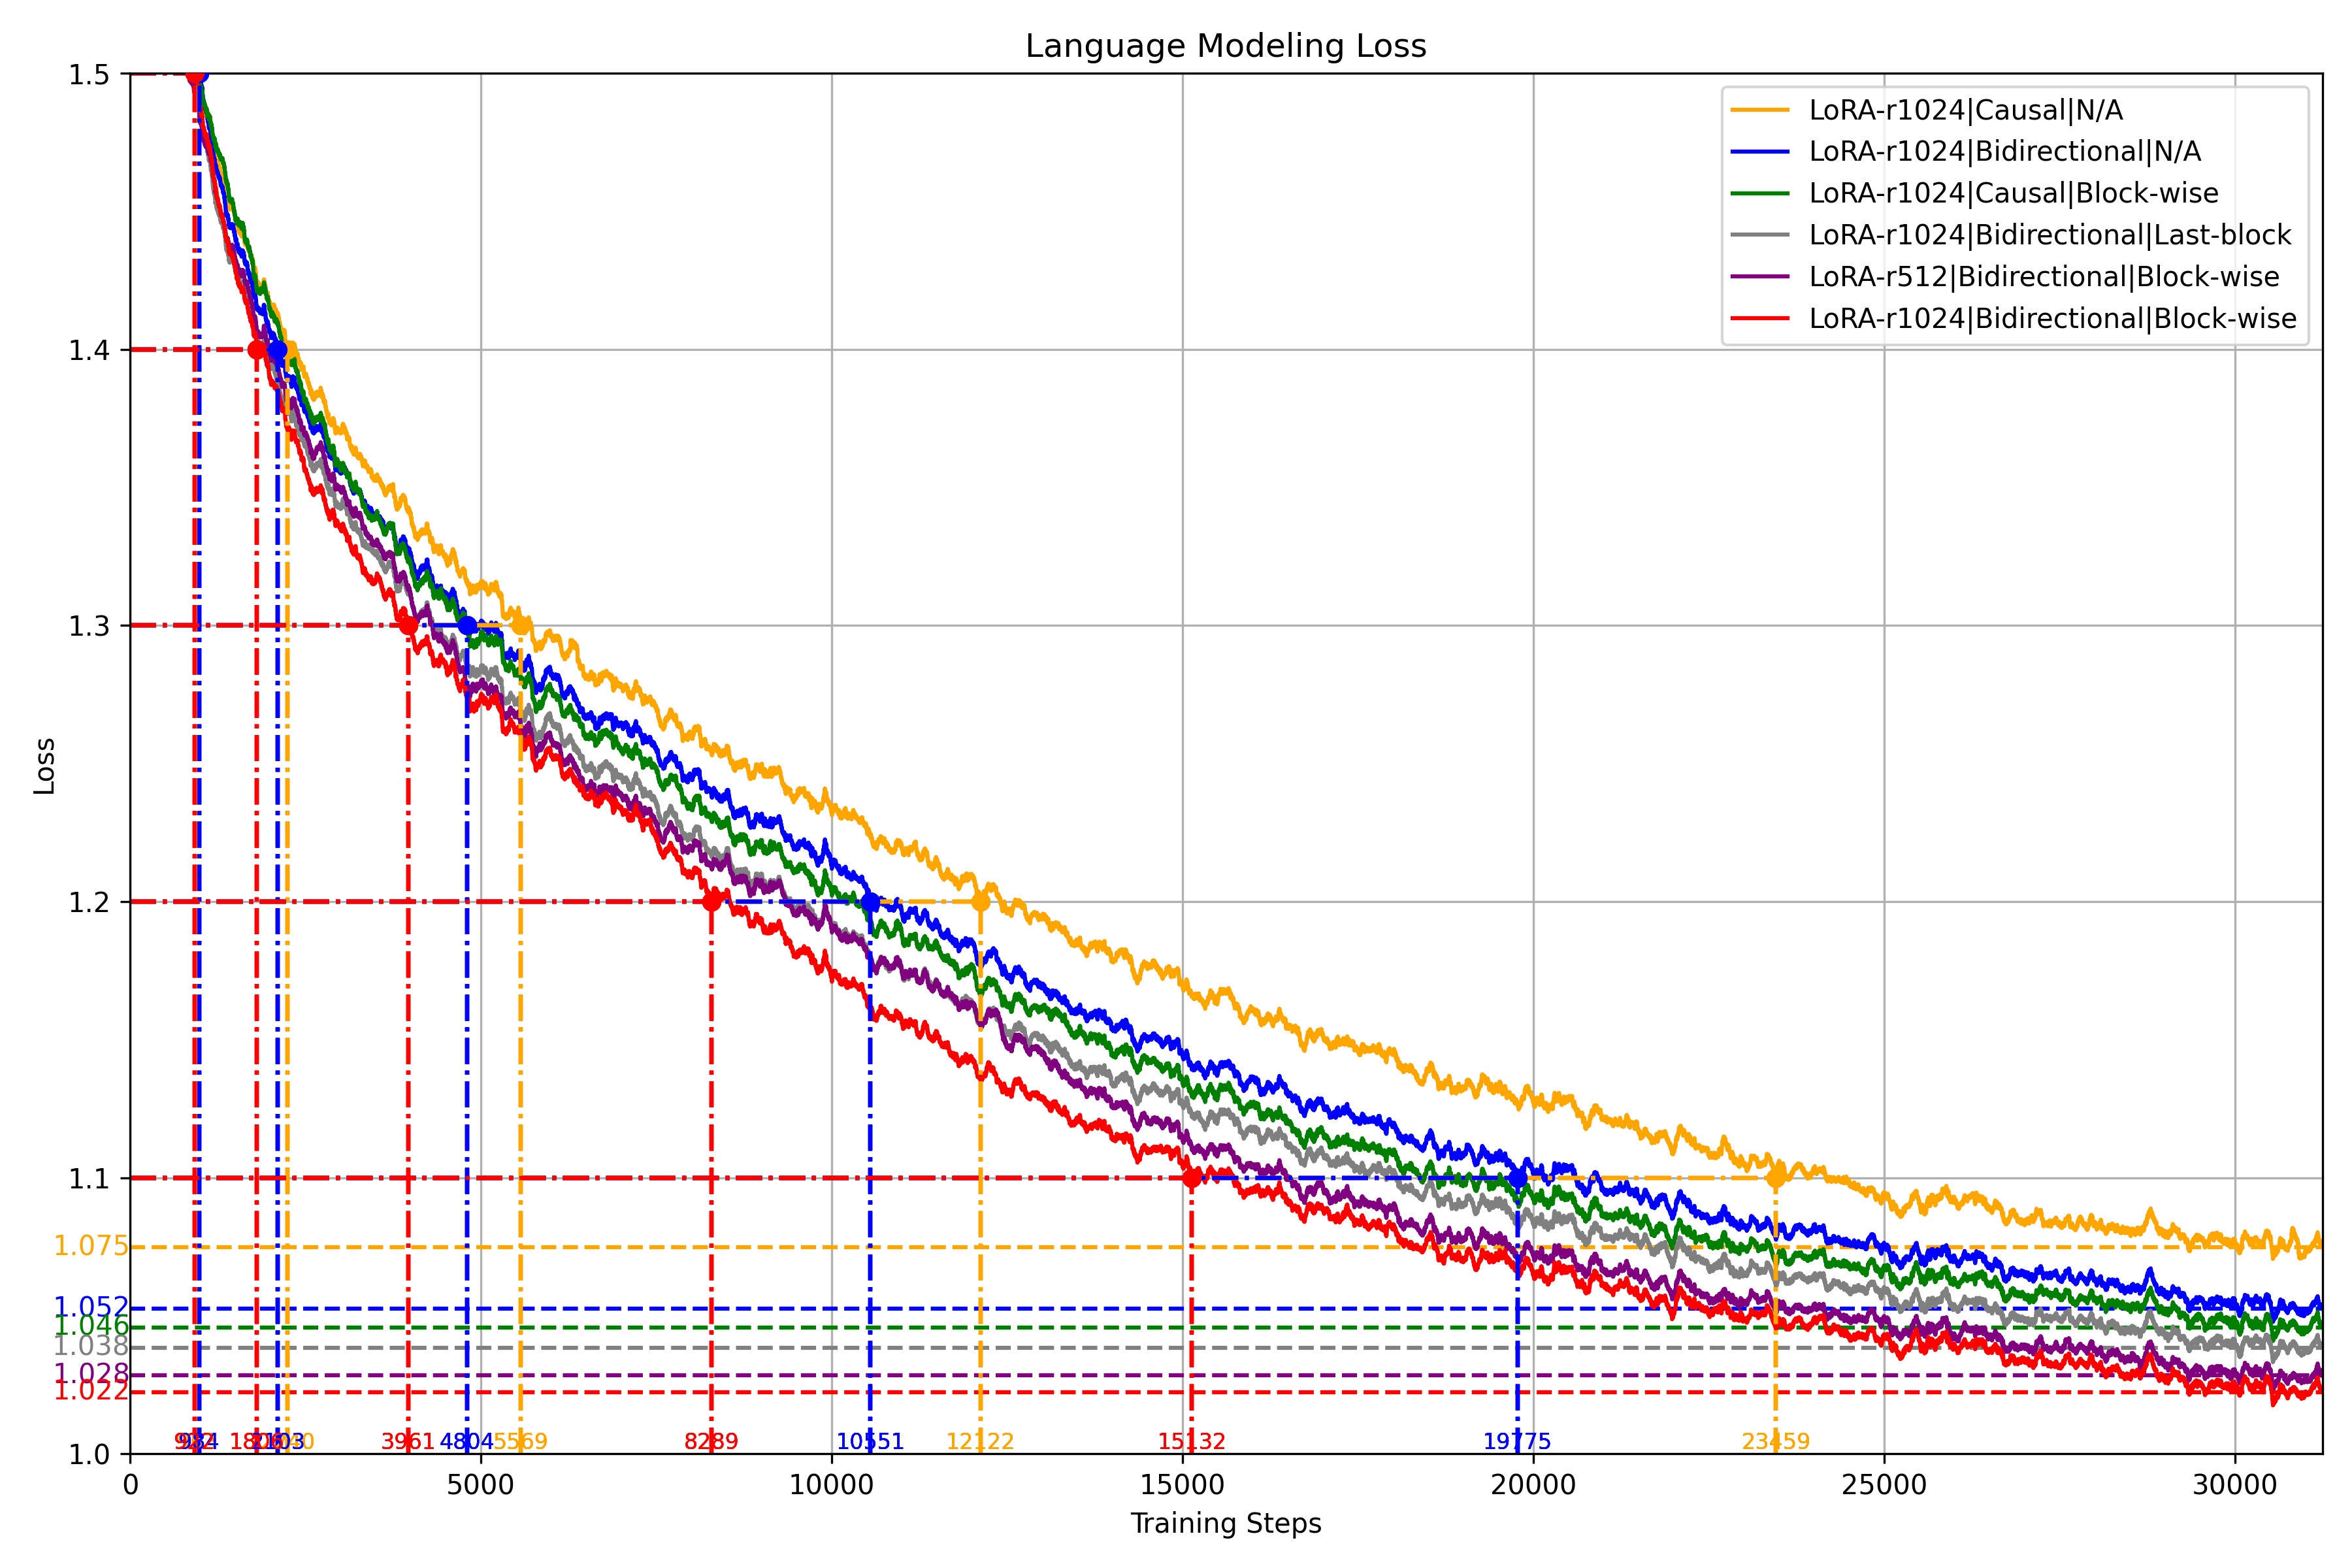
\includegraphics[width=\linewidth]{images/ablation_loss.png}
    \caption{Pre-training loss curves under different configurations. Loss values are smoothed (window=100) for visual clarity. The data sampling order was fixed to ensure fair comparison, as evidenced by the similar trajectories of the loss curves in various settings. LoRA-r1024\textbar Bidirectional\textbar Block-wise refers to the setting: LoRA with rank 1024, bi-directional attention masks for vision, and block-wise distillation. The configuration with the lowest loss was adopted as the default setting in our experiments.}
    \label{fig:ablation_loss}
\end{figure*}
\begin{figure}
    \centering
    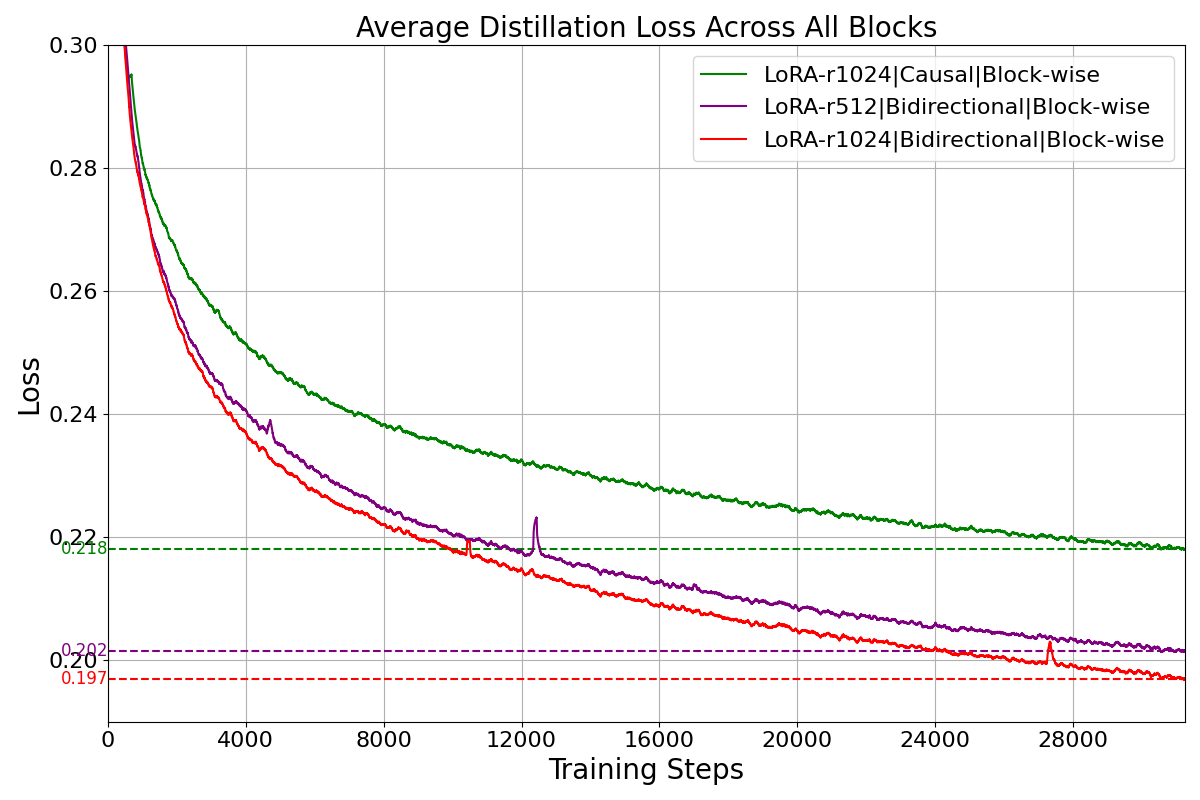
\includegraphics[width=\linewidth]{images/aux_loss_ablation.png}
    \caption{Average distillation loss across all blocks under various settings. Our LoRA-r1024\textbar Bidirectional\textbar Block-wise configuration achieves the lowest average distillation loss across all blocks. This indicates a closer alignment with the ViT’s feature space, confirming that bi-directional attention masks and a larger rank of LoRA layers also enhance visual knowledge transfer.}
    \label{fig:aux_loss}
\end{figure}
% \begin{figure}
%     \centering
%     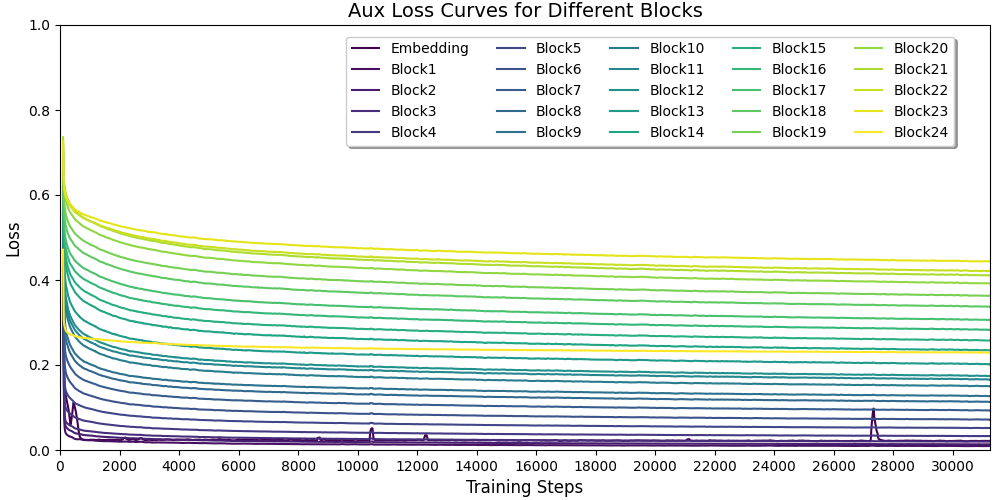
\includegraphics[width=\linewidth]{images/aux_loss.png}
%     \caption{Auxiliary loss for different blocks. loss initially increases with layer depth before declining in later blocks.}
%     \label{fig:aux_loss}
% \end{figure}
\begin{table*}[h]
    \centering
    \renewcommand{\arraystretch}{1.5} % 行间距
    \setlength{\tabcolsep}{3.5pt} % 减少列间距
    \small
    \begin{tabular}{l|c|c|cccccccc|c}
    \toprule
    Vision Params & Visual Attention Mask & Distillation type & TQA & POPE & $\mathrm{MME_p}$ & MMB & SEED-I & MMVet & AI2D & RQA & Avg.\\ 
    \midrule
    % Full LLM (7B) & Causal & N.A. & N.A. & - & - & - & - & - & - & - & - & - \\
    LoRA-r1024 (2B) & Causal & N.A. & 43.7 & 78.6 & 1137.7 & 47.7 & 57.8 & 20.6 & 49.9 & 49.7 & 50.6 \\
    LoRA-r1024 (2B) & Bidirectional & N.A. & 43.6 & 80.9 & 1132.8 & 49.1 & 58.7 & 17.9 & 47.2 & 51.5 & 50.7 \\
    LoRA-r1024 (2B) & Causal & Block-wise & 45.1 & 82.7 & 1172.9 & 52.9 & 63.7 & 20.1 & 50.9 & 51.2 & 53.2 \\
    LoRA-r1024 (2B) & Bidirectional & Last-block & 44.6 & 82.5 & 1197.5 & 51.8 & 63.8 & 17.9 & 49.9 & 52.8 & 52.9 \\
    % LoRA-r1024 (2B) & Bidirectional & Block-wise & AIMv2-Large & - & - & - & - & - & - & - & - & - \\
    LoRA-r512 (1B) & Bidirectional & Block-wise & 47.2 & 83.3 & 1280.5 & 57.6 & 65.3 & 18.5 & 55.9 & 53.1 & 55.6 \\
    % LoRA-r1536 (3B) & Bidirectional & Block-wise & AIMv2-Huge & - & - & - & - & - & - & - & - & - \\
    % LoRA-r1024 (2B) & Bidirectional & Block-wise & Detail & 49.4 & - & - & - & - & - & - & 55.1 & 57.9 \\
    LoRA-r1024 (2B) & Bidirectional & Block-wise & 50.1 & 83.8 & 1224.5 & 53.7 & 65.1 & 22.8 & 52.1 & 55.8 & 55.6 \\
    \bottomrule
    \end{tabular}
    \caption{The performance of various settings on standard benchmarks reveals that lower loss during pre-training correlates with better performance. ``LoRA-r1024 (2B)" indicates that the rank for the LoRA layers is set to 1024, with approximately 2 billion parameters unfrozen for training in total.}
    \label{tab:ablation}
\end{table*}
\begin{figure}
    \centering
    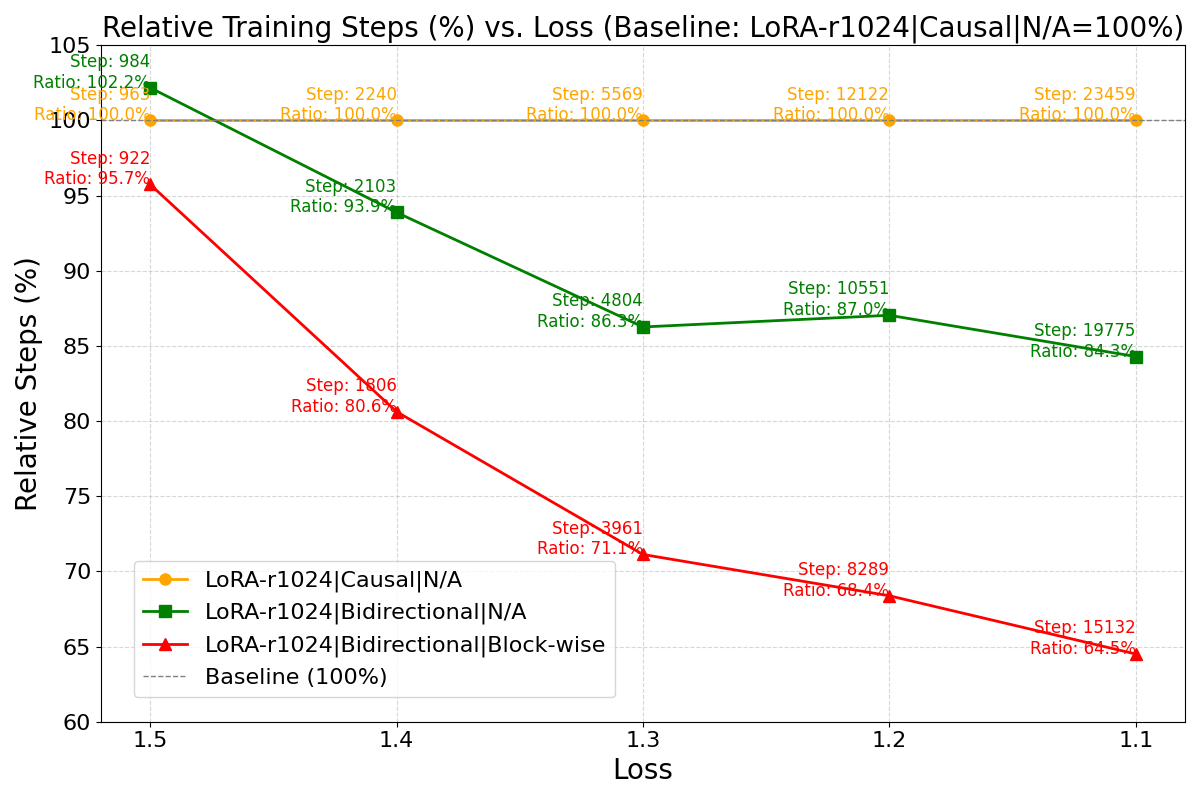
\includegraphics[width=\linewidth]{images/loss_vs_steps.png}
    \caption{Data efficiency analysis. Our experiments demonstrate that combining bi-directional attention masks for vision tokens with block-wise knowledge distillation significantly improves data efficiency compared to the vanilla LoRA configuration. Furthermore, as the target loss decreases (e.g., from 1.5 to 1.1), the required data proportion relative to the baseline diminishes progressively, indicating higher data efficiency.}
    \label{fig:loss_vs_steps}
\end{figure}
Our ablation studies focused on three key components of \model{}: vision as LoRA, block-wise distillation, and bi-directional attention masks for vision. We employed two primary methods to assess performance in various settings: the pre-training loss on an 8M subset of our DataComp29M-recap dataset, as illustrated in Figure \ref{fig:ablation_loss}, and metrics from eight benchmarks, presented in Table \ref{tab:ablation}. Additionally, we visualized the average distillation loss across all blocks, as shown in Figure \ref{fig:aux_loss}.
\\
\textbf{Ablation on vision as LoRA.} Training the full-parameter LLM proved unstable due to modality conflicts (Figure \ref{fig:full_llm}), consistent with findings in \cite{eve}. While reducing the learning rate to a lower value allowed us to observe one successful training case among several attempts, the loss decreased more slowly than that of LoRA-1024. Therefore, we have excluded it from our primary experiments.

Next, we analyzed different LoRA rank configurations in \model{}. Figure \ref{fig:ablation_loss} shows that a rank of 512 resulted in a slightly higher loss (+0.006) compared to rank 1024. This trend continued in the distillation loss (Figure \ref{fig:aux_loss}), where rank 512 showed a modestly higher average block-wise distillation loss (+0.005) compared to rank 1024. Although both configurations ended up with the same average score of 55.6 (Table \ref{tab:ablation}), the consistent loss advantage suggested that higher ranks might have better optimization potential. Furthermore, we experienced training instability with rank 1536, which prompted us to choose rank 1024 as the default configuration.
\\
\textbf{Ablation on bi-directional attention masks.} 
As demonstrated in Figure~\ref{fig:ablation_loss}, under fixed hyperparameters (e.g., LoRA rank and distillation type), the bi-directional attention mask consistently achieved lower training loss compared to causal masking. This empirical advantage was further supported by the reduced average distillation loss across all Transformer blocks, as depicted in Figure~\ref{fig:aux_loss}. Quantitatively, as evidenced in Table~\ref{tab:ablation}, replacing causal masking with bi-directional masks yielded significant performance improvements. For instance, switching from LoRA-r1024\textbar Causal\textbar Block-wise to LoRA-r1024\textbar Bidirectional\textbar Block-wise led to a 2.4-point average score gain, while replacing LoRA-r1024\textbar Causal\textbar N/A with LoRA-r1024\textbar Bidirectional\textbar N/A yielded a gain of 0.1 points.  
\\
\textbf{Block-wise distillation.} As shown in Figure~\ref{fig:ablation_loss} and Table~\ref{tab:ablation}, applying distillation to the final Transformer block alone significantly improved training efficiency. For example, the transition from the configuration LoRA-r1024\textbar{}Bidirectional\textbar{}N/A to LoRA-r1024\textbar{}Bidirectional\textbar{} Last-block yielded a 2.7-point score gain and a 0.016 reduction in loss. Extending distillation to all blocks via block-wise supervision further enhanced performance: compared with LoRA-r1024\textbar{}Bidirectional\textbar{}Last-block, LoRA-r1024\textbar{}Bidirectional\textbar{}Block-wise produced an additional 2.7-point gain and 0.016 loss reduction. These results indicated that the vanilla distillation method, i.e., last-block distillation, could accelerate training, and block-wise distillation could even strengthen this effect.
\\
% \textbf{Data strategy.} We also examined the impact of using detailed versus standard caption data during the early training stage. As shown in Table \ref{tab:ablation}, employing detailed captions for early-stage pre-training was suboptimal compared to using standard captions. This might be due to the rich and intricate visual clues present in the detailed captions, which could be too fine-grained for a model lacking prior visual capabilities to effectively learn from.
% \\
\textbf{Data efficiency analysis.} We measured data efficiency by reporting the relative number of training steps required to reach certain loss thresholds, using vanilla LoRA as the baseline. 

As illustrated in Figure~\ref{fig:loss_vs_steps}, the bi-directional attention variant without distillation (LoRA-r1024\textbar{}Bidirectional\textbar{}N/A) required 102.2\% of the baseline training steps to reach Loss=1.5, whereas adding block-wise distillation (LoRA-r1024\textbar{}Bidirectional\textbar{}Block-wise) reduced this to 95.7\%. The efficiency gap became more pronounced at lower loss: at Loss=1.1, the same configurations needed 84.3\% and 64.5\% of the vanilla LoRA baseline steps, respectively. This demonstrated that our optimal configuration achieved equivalent convergence with 35.5\% fewer training steps than vanilla LoRA.

Furthermore, the ratio of data needed by our best configuration relative to vanilla LoRA decreased over time, implying that comparable performance could be achieved with $N\times$ fewer training data.
\subsection{Standard evaluation}
\begin{table*}[h]
    \centering
    \renewcommand{\arraystretch}{1.5} % 减少行间距
    \setlength{\tabcolsep}{0.6pt} % 减少列间距
    \footnotesize % 或者使用 \footnotesize
    \begin{tabular}{llccccccccccccccccc}
        \toprule
        \multirow{2}{*}{Method} & \multirow{2}{*}{LLM} & \multirow{2}{*}{ViT} & \multicolumn{2}{c}{\# Sample} & \multirow{2}{*}{VQAv2} & \multirow{2}{*}{SQA-I} & \multirow{2}{*}{TQA} & \multirow{2}{*}{POPE} & \multirow{2}{*}{$\mathrm{MME_p}$} & \multirow{2}{*}{$\mathrm{MME_c}$} & \multirow{2}{*}{MMB} & \multirow{2}{*}{SEED-I} & \multirow{2}{*}{MMVet} & \multirow{2}{*}{AI2D} & \multirow{2}{*}{RQA} & \multirow{2}{*}{MMMU}\\
        \cmidrule{4-5}
        & & & Pretrain & Finetune & & & & & & & & & & \\
        \midrule
        % 在这里添加数据行
        \textit{Encoder-based}\\
        \midrule
        \rowcolor{gray!30}  
        BLIP2 \cite{blip2} & Vicuna-13B & EVA-1B & 129M & - & 65.0 & 61 & 42.5 & 85.3 & 1293.8 & - & - & 49.7 & 22.4 & - & - & - \\
        \rowcolor{gray!30}  
        InstructBLIP \cite{instructblip} & Vicuna-7B & EVA-1B & 129M & 1.2M & - & 60.5 & 50.1 & - & - & - & 36 & 58.8 & 26.2 & - & - & - \\
        \rowcolor{gray!30}  
        InstructBLIP \cite{instructblip} & Vicuna-13B & EVA-1B & 129M & 1.2M & - & 63.1 & 50.7 & 78.9 & 1212.8 & - & - & - & 25.6 & - & - & - \\
        LLaVA-1.5 \cite{llava1_5} & Vicuna-7B & CLIP-0.3B & 558K & 665K & 78.5 & 66.8 & 58.2 & 85.9 & 1510.7 & 316.1 & 64.3 & 66.1 & 31.1 & 54.8 & 54.8 & 35.3\\
        % LLaVA-1.5 \cite{aimv2} & Vicuna-7B & AIMv2-0.3B & 8M & 665K & vqav2 & sqa-i & tqa & pope & mmep & mmec & mmb & seed-i & mmvet & ai2d & rqa & mmmu\\
        LLaVA-1.5 \cite{llava1_5} & Qwen2.5-7B & AIMv2-0.6B & 558K & 665K & 82.3 & 77.5 & 59.2 & 85.2 & 1582.3 & 313.0 & 66.3 & 70.6 & 33.7 & 63.7 & 60.0 & 35.3\\
        \midrule
        \textit{Encoder-free}\\
        \midrule
        % \model{} & Qwen2.5-7B & \sout{AIMv2-0.6B} & 8M & 665K & vqav2 & sqa-i & tqa & pope & mmep & mmec & mmb & seed-i & mmvet & ai2d & rqa & mmmu\\
        % \model{} & Qwen2.5-7B & \sout{AIMv2-0.6B} & 8M & 665K & vqav2 & sqa-i & 50.1 & 83.8 & 1224.5 & 274.6 & 53.7 & 65.1 & 22.8 & 52.1 & 55.8 & \\
        \model{} & Qwen2.5-7B & \sout{AIMv2-0.6B} & 30M & 665K & 76.0 & 75.9 & 56.3 & 84.5 & 1363.4 & 311.1 & 64.2 & 67.5 & 33.7 & 65.6 & 57.7 & 32.2\\
       \model{}-AnyRes & Qwen2.5-7B & \sout{AIMv2-0.6B} & 30M & 665K & 76.0 & 72.0 & 58.7 & 85.5 & 1336.1 & 319.3 & 61.3 & 68.9 & 33.7 & 61.1 & 60.1 & 32.0\\
       EVE \cite{eve} & Vicuna-7B & \sout{CLIP-0.3B} & 49M(2) & 665K & 75.4 & 63.0 & 51.9 & 83.6 & 1217.3 & 266 & 49.5 & 61.3 & 25.6 & 48.5 & - & - \\
   \rowcolor{gray!30} 
      EVE-HD \cite{eve} & Vicuna-7B & \sout{CLIP-0.3B} & 49M(2) & 1.8M & 74.2 & 64.9 & 56.8 & 85.0 & 1305.7 & 322 & 52.3 & 64.6 & 25.7 & 61.0 & - & - \\
    \rowcolor{gray!30}  
      EVEv2 \cite{evev2} & Qwen2.5-7B & - & 87M(2) & 22.3M(2) & - & 96.2 & 71.1 & 87.6 & - & - & 66.3 & 71.4 & 45.0 & 74.8 & 62.4 & 39.3 \\
  \rowcolor{gray!30}  
      Mono-InternVL \cite{monointernvl} & Intern1.5-2B & - & 1.2B(2) & 150M(2) & - & 93.6 & 72.6 & - & - & - & 65.5 & 67.4 & 40.1 & 68.6 & - & 33.7 \\
      Mono-InternVL \cite{monointernvl} & Intern1.5-2B & - & 922M & 665K & - & 57 & 49 & - & 1100 & - & - & - & - & 42 & - & - \\
    Mono-InternVL \cite{monointernvl} & Intern1.5-2B & - & 1.2B(2) & 665K & - & 58 & 55 & - & 1110 & - & - & - & - & 46 & - & - \\
        \bottomrule
    \end{tabular}
    \caption{Comparison with previous methods on several benchmarks. Since this paper aims to demonstrate that \model{} is a strong base model, we did not scale the fine-tuning data. Therefore, we did not compare with recent state-of-the-art models that often require additional data engineering or involve proprietary datasets; methods that utilize extra fine-tuning data are grayed out. We classified domain-specific VQA data as fine-tuning data rather than pre-training data for EVEv2 and Mono-InternVL, which differs from their original classification in the respective papers. The notation ``49M(2)" indicates that this method employs a two-stage training process using a total of 49M image-text pairs. The strikethrough notation \sout{ViT} means that ViT is excluded during inference.}
    \label{tab:mlm_comparison}
\end{table*}
To ensure a fair comparison between \model{} and existing methods, we deliberately restricted our experimental design. While prior works (e.g., EVE, EVEv2 \cite{evev2}, and Mono-InternVL \cite{monointernvl}) have leveraged massive in-domain datasets (Table~\ref{tab:mlm_comparison}), such approaches complicated direct comparisons due to proprietary training data. Our goal is not to pursue state-of-the-art performance on benchmarks but to validate a novel MLLM architecture. Thus, we limited fine-tuning to the publicly available LLaVA-665K dataset without additional scaling.

To eliminate the potential advantages provided by LLMs and ViTs, we also trained a LLaVA-1.5 model using Qwen-2.5-7B and AIMv2-0.6B. As shown in Table~\ref{tab:mlm_comparison}, prior encoder-free methods often adopted intricate multi-stage pipelines involving module freezing strategies and proprietary datasets (e.g., 100M–1.2B samples). In contrast, our framework employed a streamlined single-stage training process (pre-training followed by fine-tuning), using about 30M image-text pairs. 
% In contrast to the claims made in EVEv2 \cite{evev2} and Mono-InternVL \cite{monointernvl}, we classified domain-specific VQA data in Table \ref{tab:mlm_comparison} as fine-tuning data rather than pre-training data, aligning with the community's consensus. 

As shown in Table~\ref{tab:mlm_comparison}, \model{} achieved performance comparable to both official and reproduced LLaVA-1.5 baselines on most benchmarks when evaluated under strict LLaVA-1.5 protocols \cite{llava1_5}, i.e., identical prompts/generation parameters. However, \model{} underperformed on MME Perception, a gap we attribute to limited world knowledge in our pre-training data. This was further quantified in Table~\ref{tab:world_knowledge}, where \model{} struggled with tasks demanding intensive world-knowledge: 1) inferring movie details from posters, 2) identifying celebrities, 3) recognizing landmarks, and 4) classifying artworks, as these tasks required external domain knowledge absent in our training datasets.

\begin{table}[]
    \centering
    \renewcommand{\arraystretch}{1.5}
    \small
    \setlength{\tabcolsep}{3pt}
    \begin{tabular}{c|cccc|c}
    \toprule
        Method & Posters & Celebrity & Landmark & Artwork & Total\\
        \midrule
        LLaVA-1.5 & 156.1 & 143.5 & 173.5 & 134.0 & 607.1\\
        \midrule
        VoRA & 117.3 & 111.2 & 139.3 & 105.5 & 473.3\\
        VoRA-AnyRes & 110.2 & 104.7 & 138.0 & 110.8 & 463.7\\
    \bottomrule
    \end{tabular}
    \caption{The performance of VoRA in world knowledge tasks. We acknowledge its deficiency, as expected, due to the lack of relevant in-domain data in our pre-training dataset. This is the primary reason for our lower performance on the MME Perception benchmark.}
    \label{tab:world_knowledge}
\end{table}